\documentclass[10pt]{beamer}

\usetheme{metropolis}
\usepackage{appendixnumberbeamer}

\usepackage{booktabs}
\usepackage[scale=2]{ccicons}

\usepackage{pgfplots}
\usepgfplotslibrary{dateplot}

\usepackage{xspace}
\newcommand{\themename}{\textbf{\textsc{metropolis}}\xspace}

\title{Metropolis}
\subtitle{A modern beamer theme}
\date{\today}
\author{Matthias Vogelgesang}
\institute{Center for modern beamer themes}
\titlegraphic{\hfill
\includegraphics[height=1.5cm]{logo.pdf}}

\begin{document}

\maketitle

\begin{frame}{Table of contents}
  \setbeamertemplate{section in toc}[sections numbered]
  \tableofcontents[hideallsubsections]
\end{frame}
%---------------------------------------------------------------------------------
%-----------------------Taylor-series Method--------------------------------------
%---------------------------------------------------------------------------------
\section{Taylor-series Method}

\begin{frame}{Taylor-series Method}
	We are given:
  $$ r_{i,1}^2=cd_{i,1}=r_{i}-r_{1} $$
  Linearize above equation by Taylor-series expansion and then solve iteratively:
	\begin{itemize}
    \item Compute position deviation
    \item Add position deviation to initial guess
    \item Solve again until deviation is considerably small
  \end{itemize}
  \alert{Convergence is not guaranteed}
\end{frame}


\begin{frame}{Taylor-series Method}
	The position deviation is computed by:
   $$\begin{bmatrix} \Delta x \\ \Delta y \end{bmatrix} = (G_{t}^T Q^{-1} G_{t})^{-1} G_{t}^T Q^{-1} h_{t}$$
  where $h_{t}$ and $G_{t}$ are given as follows
 \begin{align}
    h_{t} &= \begin{bmatrix} r_{2,1} - (r_{2}-r_{1}) \\  r_{3,1} - (r_{3}-r_{1})\\  \quad\\  r_{M,1} - (r_{M}-r_{1}) \end{bmatrix}  \\
    G_{t} &= \begin{bmatrix} (x_{1}-x)/r_{1} - (x_{2}-x)/r_{2} & (y_{1}-y)/r_{1} - (y_{2}-y)/r_{2} \\ (x_{1}-x)/r_{1} - (x_{2}-x)/r_{3} & (y_{1}-y)/r_{1} - (y_{3}-y)/r_{3}\\  \quad\\ (x_{1}-x)/r_{1} - (x_{M}-x)/r_{M} & (y_{1}-y)/r_{1} - (y_{M}-y)/r_{M} \end{bmatrix}
  \end{align}

\end{frame}
%--------------------------end--------------------------------------------------------

%-------------------------------------------------------------------------------------
%------------------------Spherical Interpolation Method-------------------------------
%-------------------------------------------------------------------------------------
\section{Spherical-Interpolation Method}

% page 1
\begin{frame}{The Equation-Error Formulation}
  We first map the spatial origin to an arbitrary sensor j, this gives:
  $$ \underline{x}_{j}\triangleq \underline{0}\Longrightarrow \begin{cases} R_{j} &= \ 0 \\ D_{j} &= \ R_{s} \end{cases}$$
  From the Pythagorean theorem, we have:
  $$(R_{s}+d_{ij})^2 = R_{i}^2 - 2\underline{x}_{i}^T \underline{x}_{s} + R_{s}^2 $$
  which is also:
  $$ 0 = R_{i}^2 - d_{ij}^2 -2R_{s}d_{ij} - 2\underline{x}_{i}^T \underline{x}_{s} $$
  \begin{center}
  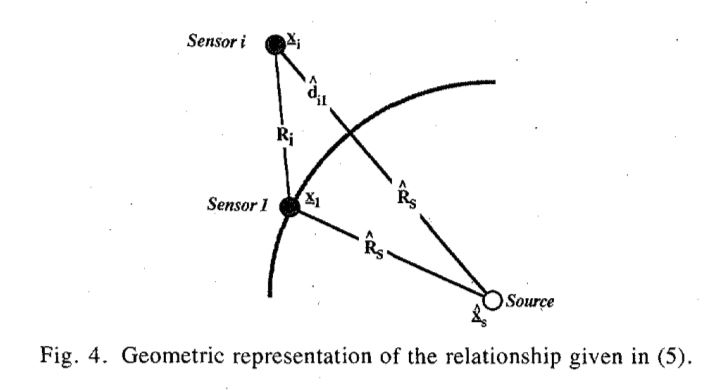
\includegraphics[scale=0.7]{Pythagorean.JPG}
  \end{center}
\end{frame}
% page 2
\begin{frame}{The Equation-Error Fomulation}
  If we take the first sensor as origin, i.e. $j=1$ \\
  As the delays are typically not measured precisely, we introduce "equation error"
  $$ \epsilon_{i} = R_{i}^2 - d_{ij}^2 -2R_{s}d_{ij} - 2\underline{x}_{i}^T \underline{x}_{s} \quad (i=2,3,\ldots,N) $$
  where $\epsilon_{i}$ is to be minimized.
  With N-1 measurements, this equation can be written in matrix notaion:
  $$ \underline{\epsilon} = \underline{\sigma} - 2R_{s}\underline{d} - 2S\underline{x}_{s} $$
  where
  \begin{align*}
    \underline{\sigma}\triangleq \begin{bmatrix} R_{2}^2 - d_{21}^2 \\ R_{3}^2 - d_{31}^2 \\ \vdots \\ R_{N}^2 - d_{N1}^2 \end{bmatrix} \qquad
    \underline{d}\triangleq \begin{bmatrix} d_{21}\\ d_{31} \\ \vdots \\ d_{N1} \end{bmatrix} \qquad
    \textbf{S} \triangleq \begin{bmatrix} x_2 & y_2 \\x_3 & y_3\\ \vdots & \vdots \\ x_N & y_N \end{bmatrix}
  \end{align*}
\end{frame}
% page 3
\begin{frame}{The Spherical-Interpolation Method}
  The formal least-squares solution for $\underline{x}_s$ \alert{given} $R_s$ is
  $$ \underline{x}_s = \frac{1}{2} S_W^* (\underline{\sigma} - 2R_s\underline{d})$$
  where
  $$  S_W^* \triangleq (S^T S)^{-1}S^T $$
  The \alert{SI} method is to minimize the equation error agian with respect to $R_s$.
  i.e. rewriting the equation error to eliminate $\underline{x}_s$ by substituting it with $R_s$, yielding a new equation error $\underline{\epsilon}^{'}$ which is linear in $R_s$:
  \begin{align*}
   \underline{\epsilon}^{'} &= \underline{\sigma} - 2R_s\underline{d} - S S^*_W (\underline{\epsilon} - 2R_s\underline{d})\\
                            &= (I - S S_W^*)(\underline{\epsilon} - 2R_s\underline{d})
  \end{align*}
  We notice that the formal least-squares estimate of  $\underline{x}_s$ \alert{given} $R_s$ is itself \textsc{linear} in $R_s$. When the minimizing $R_s$ value is found
  in this new equation, the corresponding value of $\underline{x}_s$ is automatically a minimizer of the squared equation-error norm.
\end{frame}
% page 4
\begin{frame}{The Spherical-Interpolation Method}
  The solution is given by
  $$ \tilde{R}_s = \frac{\underline{d}^T P_s^{\bot}V P_s^{\bot}\underline{\sigma}}{2\underline{d}^T P_s^{\bot} V P_s^{\bot}\underline{d}}$$
  where $P_s^{\bot}$ is defined as
  $$P_s^{\bot} \triangleq I - SS_W^*$$
  Substituting this solution into
  $$ \underline{x}_s = \frac{1}{2} S_W^* (\underline{\sigma} - 2R_s\underline{d})$$
  yields the source location estimate
  $$ \hat{\underline{x}}_s = \frac{1}{2} (S^T W S)^{-1} S^T W (I - \frac{\underline{d}\ \underline{d}^T P_s^{\bot} V P_s^{\bot}} {\underline{d}^T P_s^{\bot} V P_s^{\bot} \underline{d}}) \underline{\sigma}$$
\end{frame}
% page 5
\begin{frame}{The Spherical-Interpolation Method}
  When $W = V$ , this estimator is the minimizer of the weighted norm of the \alert{projected} equation error
  $$ Z_{\underline{x}_s} = \underline{\epsilon}^T P_{\underline{d}}^{\bot} W P_{\underline{d}}^{\bot} \underline{\epsilon} $$
  Minimizing $Z_{\underline{x}_s}$, one gets a simplified expression of the estimator
  $$ \hat{\underline{x}}_s = \frac{1}{2} (S^T  P_{\underline{d}}^{\bot} W P_{\underline{d}}^{\bot} S)^{-1} S^T P_{\underline{d}}^{\bot} \underline{\sigma} $$
  By now, the \alert{Maximum Likelihood Estimation} of the $\underline{x}_s$ is obtained.
  \vfill
  \textsc{in simulation:\\}
  The weighting matrices $\textbf{W}$ and $\textbf{V}$ are both set to $\textbf{Q}^{-1}$
\end{frame}
%-----------------------------------------end-----------------------------------------

%-------------------------------------------------------------------------------------
%----------------------------------------CRLB-----------------------------------------
%-------------------------------------------------------------------------------------
\section{Cram\'{e}r-Rao Lower Bound}

% page 1
\begin{frame}{Cram\'{e}r-Rao Lower Bound}
  In the simplest form, the CRLB states that the variance of any unbiased estimator
  is no smaller than the inverse of the Fisher information matrix.
   $$\textbf{var}(\hat{\theta}) \geqslant \textbf{J}(\theta)^{-1} $$
  It is derived from the \textsc{appendix} that the CRLB of the localization problem
  is given by
   $$ \Phi^0 = c^2 (\textbf{G}_t^{0T} \textbf{Q}^{-1} \textbf{G}_l^0)^{-1} $$
  Also, it is proved that the proposed method with arbitrary sensor array can achieve CRLB,
  therefore, one can use the following method to compute the lower bound of covariance matrix
  \begin{align*}
    \Phi^0 &= \text{cov}(\textbf{z}_p) = \frac{1}{4} \textbf{B}^{''-1} \text{cov} (\textbf{z}_a^{'}) \textbf{B}^{''-1} \\
           &= c^2 ( \textbf{B}^{''} \textbf{G}_a^{'T} \textbf{B}^{'-1} \textbf{G}_a^{0T} \textbf{B}^{-1} \textbf{Q}^{-1} \textbf{B}^{-1} \textbf{G}_a^{0}  \textbf{B}^{'-1} \textbf{G}_a^{'} \textbf{B}^{''} )^{-1}
  \end{align*}
  which is the covariance matrix of $\textbf{z}_p$ when errors are ignored.
  \begin{center}
    \textsc{Predefined matrices are given in the next slide}
  \end{center}
\end{frame}
% page 2
\begin{frame}{Cram\'{e}r-Rao Lower Bound}
  \begin{equation*}
    \Phi^0 = c^2 ( \textbf{B}^{''} \textbf{G}_a^{'T} \textbf{B}^{'-1} \textbf{G}_a^{0T} \textbf{B}^{-1} \textbf{Q}^{-1} \textbf{B}^{-1} \textbf{G}_a^{0}  \textbf{B}^{'-1} \textbf{G}_a^{'} \textbf{B}^{''} )^{-1}
  \end{equation*}
  where
  \begin{align*}
     \textbf{G}_a^0   &= - \begin{bmatrix} x_2  & y_2 & r_2-r_1 \\   x_3  & y_3 & r_3-r_1 \\ \vdots & \vdots & \vdots \\  x_M  & y_M & r_M-r_1 \end{bmatrix} \qquad \qquad
     \textbf{B}^{''}  = \begin{bmatrix} (x^0 - x_1) & 0 \\  0 & (y^0 - y_1)\end{bmatrix}\\
     \textbf{B}^{'}\  &= \text{diag}\{(x^0 - x_1),(y^0 - y_1),r_1^0\}\qquad
     \textbf{G}_a^{'} = \begin{bmatrix} 1 & 0 & 1 \\  0 & 1 & 1\end{bmatrix}^{'} \\
     \textbf{B}  \ \  &= \text{diag}\{r_2^0, r_3^0, \cdots r_M^0\}
   \end{align*}
   The covariance matrix of position estimate contains the uncertainty information in localization.
   In particular, the position mean-square error (\textsc{MSE}) is equal to the \alert{trace} of $\Phi$.
\end{frame}
%-----------------------------------------end-----------------------------------------











\section{Introduction}

\begin{frame}[fragile]{Metropolis}

  The \themename theme is a Beamer theme with minimal visual noise
  inspired by the \href{https://github.com/hsrmbeamertheme/hsrmbeamertheme}{\textsc{hsrm} Beamer
  Theme} by Benjamin Weiss.

  Enable the theme by loading

  \begin{verbatim}    \documentclass{beamer}
    \usetheme{metropolis}\end{verbatim}

  Note, that you have to have Mozilla's \emph{Fira Sans} font and XeTeX
  installed to enjoy this wonderful typography.
\end{frame}
\begin{frame}[fragile]{Sections}
  Sections group slides of the same topic

  \begin{verbatim}    \section{Elements}\end{verbatim}

  for which \themename provides a nice progress indicator \ldots
\end{frame}

\section{Title formats}

\begin{frame}{Metropolis title formats}
	\themename supports 4 different title formats:
	\begin{itemize}
		\item Regular
		\item \textsc{Small caps}
		\item \textsc{all small caps}
		\item ALL CAPS
	\end{itemize}
	They can either be set at once for every title type or individually.
\end{frame}

{
    \metroset{titleformat frame=smallcaps}
\begin{frame}{Small caps}
	This frame uses the \texttt{smallcaps} title format.

	\begin{alertblock}{Potential Problems}
		Be aware that not every font supports small caps. If for example you typeset your presentation with pdfTeX and the Computer Modern Sans Serif font, every text in small caps will be typeset with the Computer Modern Serif font instead.
	\end{alertblock}
\end{frame}
}

{
\metroset{titleformat frame=allsmallcaps}
\begin{frame}{All small caps}
	This frame uses the \texttt{allsmallcaps} title format.

	\begin{alertblock}{Potential problems}
		As this title format also uses small caps you face the same problems as with the \texttt{smallcaps} title format. Additionally this format can cause some other problems. Please refer to the documentation if you consider using it.

		As a rule of thumb: just use it for plaintext-only titles.
	\end{alertblock}
\end{frame}
}

{
\metroset{titleformat frame=allcaps}
\begin{frame}{All caps}
	This frame uses the \texttt{allcaps} title format.

	\begin{alertblock}{Potential Problems}
		This title format is not as problematic as the \texttt{allsmallcaps} format, but basically suffers from the same deficiencies. So please have a look at the documentation if you want to use it.
	\end{alertblock}
\end{frame}
}

\section{Elements}

\begin{frame}[fragile]{Typography}
      \begin{verbatim}The theme provides sensible defaults to
\emph{emphasize} text, \alert{accent} parts
or show \textbf{bold} results.\end{verbatim}

  \begin{center}becomes\end{center}

  The theme provides sensible defaults to \emph{emphasize} text,
  \alert{accent} parts or show \textbf{bold} results.
\end{frame}

\begin{frame}{Font feature test}
  \begin{itemize}
    \item Regular
    \item \textit{Italic}
    \item \textsc{Small Caps}
    \item \textbf{Bold}
    \item \textbf{\textit{Bold Italic}}
    \item \textbf{\textsc{Bold Small Caps}}
    \item \texttt{Monospace}
    \item \texttt{\textit{Monospace Italic}}
    \item \texttt{\textbf{Monospace Bold}}
    \item \texttt{\textbf{\textit{Monospace Bold Italic}}}
  \end{itemize}
\end{frame}

\begin{frame}{Lists}
  \begin{columns}[T,onlytextwidth]
    \column{0.33\textwidth}
      Items
      \begin{itemize}
        \item Milk \item Eggs \item Potatoes
      \end{itemize}

    \column{0.33\textwidth}
      Enumerations
      \begin{enumerate}
        \item First, \item Second and \item Last.
      \end{enumerate}

    \column{0.33\textwidth}
      Descriptions
      \begin{description}
        \item[PowerPoint] Meeh. \item[Beamer] Yeeeha.
      \end{description}
  \end{columns}
\end{frame}
\begin{frame}{Animation}
  \begin{itemize}[<+- | alert@+>]
    \item \alert<4>{This is\only<4>{ really} important}
    \item Now this
    \item And now this
  \end{itemize}
\end{frame}
\begin{frame}{Figures}
  \begin{figure}
    \newcounter{density}
    \setcounter{density}{20}
    \begin{tikzpicture}
      \def\couleur{alerted text.fg}
      \path[coordinate] (0,0)  coordinate(A)
                  ++( 90:5cm) coordinate(B)
                  ++(0:5cm) coordinate(C)
                  ++(-90:5cm) coordinate(D);
      \draw[fill=\couleur!\thedensity] (A) -- (B) -- (C) --(D) -- cycle;
      \foreach \x in {1,...,40}{%
          \pgfmathsetcounter{density}{\thedensity+20}
          \setcounter{density}{\thedensity}
          \path[coordinate] coordinate(X) at (A){};
          \path[coordinate] (A) -- (B) coordinate[pos=.10](A)
                              -- (C) coordinate[pos=.10](B)
                              -- (D) coordinate[pos=.10](C)
                              -- (X) coordinate[pos=.10](D);
          \draw[fill=\couleur!\thedensity] (A)--(B)--(C)-- (D) -- cycle;
      }
    \end{tikzpicture}
    \caption{Rotated square from
    \href{http://www.texample.net/tikz/examples/rotated-polygons/}{texample.net}.}
  \end{figure}
\end{frame}
\begin{frame}{Tables}
  \begin{table}
    \caption{Largest cities in the world (source: Wikipedia)}
    \begin{tabular}{@{} lr @{}}
      \toprule
      City & Population\\
      \midrule
      Mexico City & 20,116,842\\
      Shanghai & 19,210,000\\
      Peking & 15,796,450\\
      Istanbul & 14,160,467\\
      \bottomrule
    \end{tabular}
  \end{table}
\end{frame}
\begin{frame}{Blocks}
  Three different block environments are pre-defined and may be styled with an
  optional background color.

  \begin{columns}[T,onlytextwidth]
    \column{0.5\textwidth}
      \begin{block}{Default}
        Block content.
      \end{block}

      \begin{alertblock}{Alert}
        Block content.
      \end{alertblock}

      \begin{exampleblock}{Example}
        Block content.
      \end{exampleblock}

    \column{0.5\textwidth}

      \metroset{block=fill}

      \begin{block}{Default}
        Block content.
      \end{block}

      \begin{alertblock}{Alert}
        Block content.
      \end{alertblock}

      \begin{exampleblock}{Example}
        Block content.
      \end{exampleblock}

  \end{columns}
\end{frame}
\begin{frame}{Math}
  \begin{equation*}
    e = \lim_{n\to \infty} \left(1 + \frac{1}{n}\right)^n
  \end{equation*}
\end{frame}
\begin{frame}{Line plots}
  \begin{figure}
    \begin{tikzpicture}
      \begin{axis}[
        mlineplot,
        width=0.9\textwidth,
        height=6cm,
      ]

        \addplot {sin(deg(x))};
        \addplot+[samples=100] {sin(deg(2*x))};

      \end{axis}
    \end{tikzpicture}
  \end{figure}
\end{frame}
\begin{frame}{Bar charts}
  \begin{figure}
    \begin{tikzpicture}
      \begin{axis}[
        mbarplot,
        xlabel={Foo},
        ylabel={Bar},
        width=0.9\textwidth,
        height=6cm,
      ]

      \addplot plot coordinates {(1, 20) (2, 25) (3, 22.4) (4, 12.4)};
      \addplot plot coordinates {(1, 18) (2, 24) (3, 23.5) (4, 13.2)};
      \addplot plot coordinates {(1, 10) (2, 19) (3, 25) (4, 15.2)};

      \legend{lorem, ipsum, dolor}

      \end{axis}
    \end{tikzpicture}
  \end{figure}
\end{frame}
\begin{frame}{Quotes}
  \begin{quote}
    Veni, Vidi, Vici
  \end{quote}
\end{frame}

{%
\setbeamertemplate{frame footer}{My custom footer}
\begin{frame}[fragile]{Frame footer}
    \themename defines a custom beamer template to add a text to the footer. It can be set via
    \begin{verbatim}\setbeamertemplate{frame footer}{My custom footer}\end{verbatim}
\end{frame}
}

\begin{frame}{References}
  Some references to showcase [allowframebreaks] \cite{knuth92,ConcreteMath,Simpson,Er01,greenwade93}
\end{frame}

\section{Conclusion}

\begin{frame}{Summary}

  Get the source of this theme and the demo presentation from

  \begin{center}\url{github.com/matze/mtheme}\end{center}

  The theme \emph{itself} is licensed under a
  \href{http://creativecommons.org/licenses/by-sa/4.0/}{Creative Commons
  Attribution-ShareAlike 4.0 International License}.

  \begin{center}\ccbysa\end{center}

\end{frame}

\begin{frame}[standout]
  Questions?
\end{frame}

\appendix

\begin{frame}[fragile]{Backup slides}
  Sometimes, it is useful to add slides at the end of your presentation to
  refer to during audience questions.

  The best way to do this is to include the \verb|appendixnumberbeamer|
  package in your preamble and call \verb|\appendix| before your backup slides.

  \themename will automatically turn off slide numbering and progress bars for
  slides in the appendix.
\end{frame}

\begin{frame}[allowframebreaks]{References}

  \bibliography{demo}
  \bibliographystyle{abbrv}

\end{frame}

\end{document}
